\documentclass[11pt,a4paper]{article}

% ====== Packages ======
\usepackage[utf8]{inputenc}
\usepackage[T1]{fontenc}
\usepackage{amsmath, amssymb, amsthm}
\usepackage{graphicx}
\usepackage{geometry}
\usepackage{hyperref}
\usepackage{xcolor}
\usepackage{booktabs}
\usepackage{caption}
\usepackage{subcaption}
\usepackage{cite}
\usepackage{physics} % For bra-ket notation

% ====== Page Setup ======
\geometry{
    top=2.5cm,
    bottom=2.5cm,
    left=2.5cm,
    right=2.5cm
}

\hypersetup{
    colorlinks=true,
    linkcolor=blue,
    filecolor=magenta,      
    urlcolor=cyan,
    citecolor=red,
}

% ====== Title and Authors ======
\title{\textbf{Time Evolution of Quantum Spin Chains: Exact Diagonalisation and Trotter Simulation}}
\author{
    % TODO: Add your group members here
    Group Members \\
    \textit{School of Physics and Astronomy} \\
    \textit{The University of Edinburgh}
}
\date{\today}

\begin{document}

\maketitle

% ====== Abstract ======
\begin{abstract}
This report investigates the real-time dynamics of a one-dimensional anisotropic Heisenberg (XXZ) spin chain through a comparative study of classical and quantum simulation methodologies. We benchmark exact sparse-matrix time evolution against ideal first- and second-order Qiskit Trotter-Suzuki circuits, and further assess the impact of realistic gate-level noise using density-matrix simulations via \texttt{AerSimulator}. For a system of $L = 8$ sites, we characterise the spatiotemporal magnetisation dynamics and the momentum-frequency spectrum of the local observable $\langle Z_i(t) \rangle$. Our error scaling analysis confirms the expected $\mathcal{O}(\Delta t^p)$ algorithmic convergence of $p$-th order product formulas. However, noisy simulations reveal that modest Pauli-type gate errors rapidly induce decoherence, significantly degrading the long-time fidelity of the many-body state. These results underscore the critical interplay between algorithmic approximation and physical hardware noise in the Noisy Intermediate-Scale Quantum (NISQ) era, highlighting the stringent requirements for fault-tolerant Hamiltonian simulation.
\end{abstract}

\newpage
\tableofcontents
\newpage

% ====== 1. Introduction ======
\section{Introduction} \label{sec:intro}

The simulation of strongly interacting quantum many-body systems represents one of the most highly anticipated applications of quantum computing \cite{Georgescu2014, Daley2022}. Classical simulation methods face an exponential bottleneck: the Hilbert space dimension for a system of $L$ spin-$\frac{1}{2}$ particles scales as $2^L$, rendering exact diagonalisation and full state-vector tracking intractable for systems exceeding $L \approx 40-50$ sites even on modern supercomputers.

Richard Feynman famously proposed that simulating quantum mechanics efficiently requires a computational framework built from quantum mechanical elements themselves \cite{Feynman1982}. This insight forms the foundation of modern quantum simulation algorithms. By mapping the $2^L$-dimensional many-body state onto an $L$-qubit register, the exponential memory overhead is circumvented. Furthermore, the time-evolution operator of local Hamiltonians can be efficiently decomposed into sequences of low-depth quantum gates using product formulas, such as the Trotter-Suzuki decomposition \cite{Lloyd1996}.

The one-dimensional XXZ Heisenberg spin chain serves as a paradigmatic model in condensed matter physics, capturing the competition between symmetric exchange interactions and Ising anisotropy. Its phase diagram encompasses gapless Luttinger-liquid, ferromagnetic, and antiferromagnetic N\'eel phases. Consequently, it is an ideal testbed for evaluating the performance and fidelity of quantum algorithms.

The objectives of this project are threefold:
\begin{enumerate}
    \item \textbf{Classical Benchmarking:} To compute the exact real-time dynamics of the XXZ model for $L=8$ spins using sparse-matrix exponentiation, yielding high-resolution space-time magnetisation maps and momentum-frequency spectra.
    \item \textbf{Ideal Quantum Simulation:} To implement and validate first- and second-order Trotter-Suzuki quantum circuits in Qiskit, quantitatively assessing algorithmic truncation errors.
    \item \textbf{Noisy Circuit Assessment:} To simulate the same Trotter circuits using a realistic Pauli error model in a density-matrix formalism, isolating the effects of gate noise on the propagation of quantum correlations.
\end{enumerate}

By evaluating these three methodological tiers, this report provides a rigorous analysis of the conditions under which near-term quantum hardware-inspired models can accurately capture complex many-body dynamics, and identifies the operational thresholds where noise becomes the prohibitive limitation.

% ====== 2. Theoretical Background ======
\section{Theoretical Background} \label{sec:theory}

\subsection{The XXZ Heisenberg Spin Chain}
We consider a one-dimensional XXZ spin chain of length $L$ with open boundary conditions. The system is governed by the Hamiltonian:
\begin{equation} \label{eq:hamiltonian}
H = -\sum_{i=0}^{L-2} \left( \sigma_i^x \sigma_{i+1}^x + \sigma_i^y \sigma_{i+1}^y + J_z \sigma_i^z \sigma_{i+1}^z \right),
\end{equation}
where $\sigma_i^\alpha$ (with $\alpha \in \{x,y,z\}$) are the Pauli matrices acting on site $i$. The parameter $J_z$ is the dimensionless anisotropy coupling governing the $z$-axis interaction relative to the transverse $XY$ exchange. 

The physical characteristics of the ground state and excitations are highly dependent on $J_z$:
\begin{itemize}
    \item \textbf{Ferromagnetic Phase} ($J_z > 1$): The spins prefer to align parallel to the $z$-axis, exhibiting a finite energy gap to spin-wave excitations.
    \item \textbf{Critical Phase} ($-1 < J_z \leq 1$): A gapless Luttinger liquid phase governed by quasi-long-range order.
    \item \textbf{Antiferromagnetic N\'eel Phase} ($J_z < -1$): Spins prefer alternating anti-parallel alignment.
\end{itemize}

\subsection{Time Evolution and Observables}
The state of the system at time $t$ obeys the Schr\"odinger equation and evolves unitarily:
\begin{equation}
\ket{\psi(t)} = e^{-iHt} \ket{\psi(0)} \quad (\text{setting } \hbar = 1).
\end{equation}
To probe the dynamics, we calculate the local Pauli expectation values $\langle \sigma_i^\alpha(t) \rangle = \bra{\psi(t)} \sigma_i^\alpha \ket{\psi(t)}$ for all sites $i$. The spatiotemporal evolution of $\langle Z_i(t) \rangle$ provides insights into the ballistic spread of local excitations and the propagation of spin waves.

\subsection{Trotter-Suzuki Decomposition}
Implementing the global unitary $e^{-iHt}$ directly on a quantum computer is generally impossible because the terms in $H$ do not commute. Writing the Hamiltonian as a sum of local nearest-neighbour bond interactions $H = \sum_b H_b$, we employ the Trotter-Suzuki product formulas to approximate the evolution.

The \textbf{first-order Trotter decomposition} is given by:
\begin{equation}
e^{-iH\Delta t} = \prod_b e^{-iH_b\Delta t} + \mathcal{O}(\Delta t^2).
\end{equation}

The \textbf{second-order symmetric Trotter decomposition} achieves higher accuracy by symmetrically splitting the time step:
\begin{equation}
e^{-iH\Delta t} = \prod_b^{\rightarrow} e^{-iH_b\Delta t / 2} \prod_b^{\leftarrow} e^{-iH_b\Delta t / 2} + \mathcal{O}(\Delta t^3),
\end{equation}
where the arrows denote the ordering of the non-commuting two-site unitary gates. In our Qiskit implementation, each local term $e^{-iH_b \Delta t}$ is synthesised using native \texttt{RXX}, \texttt{RYY}, and \texttt{RZZ} gates.

% ====== 3. Quantum Noise and Decoherence ======
\section{Quantum Noise and Decoherence} \label{sec:noise}

Real-world execution of deep quantum circuits is hindered by environmental decoherence and imperfect control logic. To systematically assess hardware limitations, we introduce a phenomenological noise model to the otherwise ideal Trotter circuits.

\subsection{Pauli Error Channels}
We model gate-level imperfections as stochastic Pauli channels applied immediately after each primitive gate. Specifically, each target qubit independently undergoes:
\begin{itemize}
    \item A bit-flip (Pauli $X$) error with probability $p_X$.
    \item A phase-flip (Pauli $Z$) error with probability $p_Z$.
    \item The identity operation (no error) with probability $1 - p_X - p_Z$.
\end{itemize}
For two-qubit gates, this single-qubit error channel is applied independently to both participating qubits, assuming uncorrelated local noise \cite{Krantz2019}.

\subsection{Density-Matrix Evolution}
Under stochastic noise, the system cannot be described by a pure state vector $\ket{\psi}$. Instead, the state evolves as a statistical ensemble represented by a density matrix $\rho(t)$. The expectation value of an observable $\hat{O}$ is computed as:
\begin{equation}
\langle \hat{O}(t) \rangle = \text{Tr}[\hat{O} \rho(t)].
\end{equation}
By performing deterministic density-matrix simulations (rather than Monte Carlo trajectory sampling), we obtain the exact average dynamics of the noisy circuit without statistical shot-noise artifacts, allowing for a precise evaluation of decoherence-induced errors.

% ====== 4. Our Implementation ======
\section{Our Implementation} \label{sec:implementation}

The simulation framework developed for this project integrates three progressive levels of complexity. The full codebase relies on the \texttt{numpy}, \texttt{scipy}, and \texttt{qiskit} ecosystems.

\subsection{Exact Diagonalisation (Classical Benchmark)}
For a system of $L=8$, the $256 \times 256$ Hamiltonian is constructed using Kronecker products of Pauli matrices. To maximise computational efficiency, the operators are instantiated as SciPy \texttt{csr\_matrix} sparse arrays. The exact time evolution operator $U(\Delta t) = e^{-iH\Delta t}$ is computed using \texttt{scipy.linalg.expm}, a highly accurate matrix exponential algorithm based on Pad\'e approximations \cite{AlMohy2011}. The state vector is updated iteratively: $\ket{\psi(t+\Delta t)} = U(\Delta t)\ket{\psi(t)}$.

\subsection{Qiskit Trotter Circuit Construction}
The initial state is prepared by defining a computational basis string and applying a Hadamard ($H$) and Phase ($R_z(\pi/3)$) gate to the central site ($i=4$) to break symmetry and induce local dynamics. The Trotter circuits are dynamically generated by appending blocks of \texttt{RXX}, \texttt{RYY}, and \texttt{RZZ} gates parameterised by the time step $\Delta t$ and the coupling $J_z$. For ideal algorithmic validation, these circuits are executed using Qiskit's \texttt{Statevector} simulator. Local observables are efficiently extracted using \texttt{SparsePauliOp} contractions.

\subsection{Noisy Aer Simulation Environment}
To evaluate hardware-like conditions, the identical Trotter circuits are executed using Qiskit's \texttt{AerSimulator} configured with \texttt{method="density\_matrix"}. A custom \texttt{NoiseModel} injects the defined Pauli errors ($p_X = 0.002, p_Z = 0.006$) into the simulation pipeline. Initial state preparation is assumed ideal to strictly isolate the degradation caused by dynamical Trotterization errors compounded by gate noise.

% ====== 5. Results ======
\section{Results} \label{sec:results}

We investigate three distinct physical scenarios, distinguished by the anisotropy $J_z$ and the initial background state:
\begin{itemize}
    \item \textbf{Case A:} Ferromagnetic regime ($J_z = 1.5$), initial state $\ket{00...0}$ with site 4 rotated to the equator.
    \item \textbf{Case B:} Ferromagnetic regime ($J_z = 1.5$), initial state $\ket{11...1}$ with site 4 rotated.
    \item \textbf{Case C:} Antiferromagnetic regime ($J_z = -1.5$), alternating N\'eel state $\ket{1010...}$ with site 4 rotated.
\end{itemize}

\subsection{Classical Benchmarks: Exact Dynamics}
Figure \ref{fig:exact} displays the exact space-time dynamics of the local Pauli expectations. 
\textit{Note: The numerical heatmaps are rendered without continuous interpolation to accurately reflect the discrete spatial lattice of the $L=8$ spin chain.}

% Placeholder for Exact Dynamics Figure
\begin{figure}[h]
    \centering
    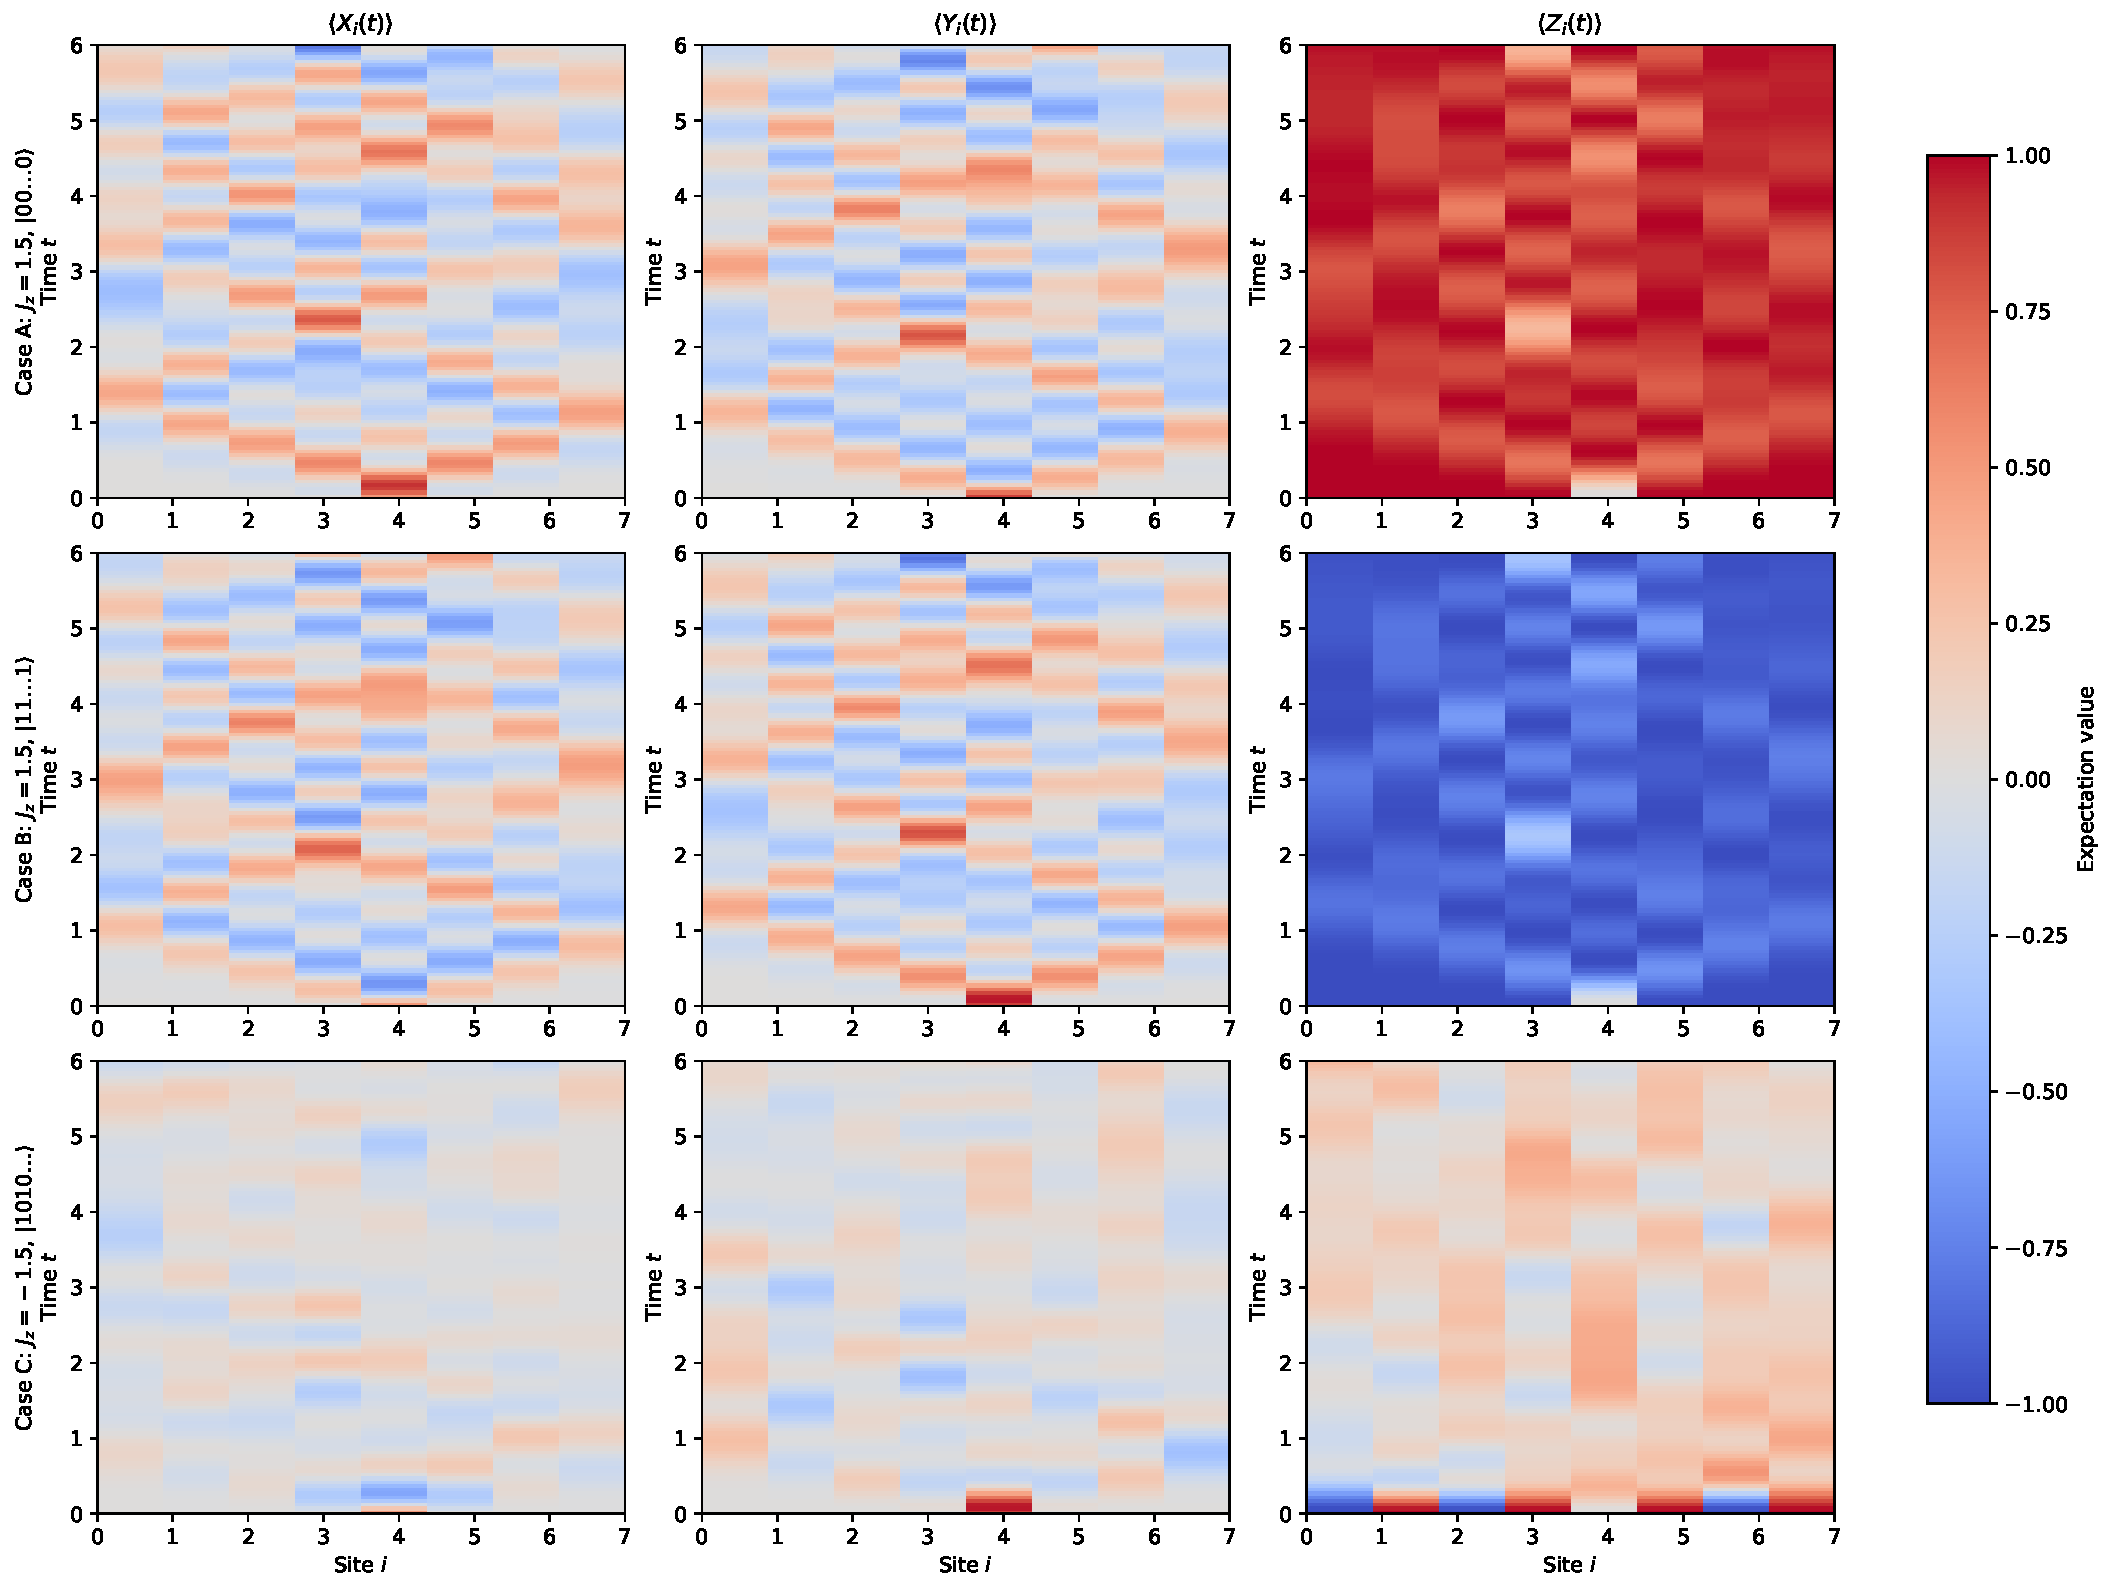
\includegraphics[width=0.9\textwidth]{figures/exact_dynamics.pdf}
    \caption{\textbf{Exact space-time dynamics of local Pauli expectations.} The propagation of the initial local excitation manifests as a light cone. In the ferromagnetic regimes (Cases A and B), the excitation is partially confined due to the energy gap. In the antiferromagnetic regime (Case C), the alternating background order strongly modulates the short-wavelength dynamics.}
    \label{fig:exact}
\end{figure}

\subsection{Quantum Simulation: Ideal Trotter Dynamics}
We simulated the dynamics using a second-order Trotter circuit with a time step of $\Delta t = 0.05$. As visually demonstrated by the vanishingly small residuals in Figure \ref{fig:trotter_error}, the algorithmic error of the second-order decomposition is practically negligible at this resolution.

% Placeholder for Trotter Error Figure
\begin{figure}[h]
    \centering
    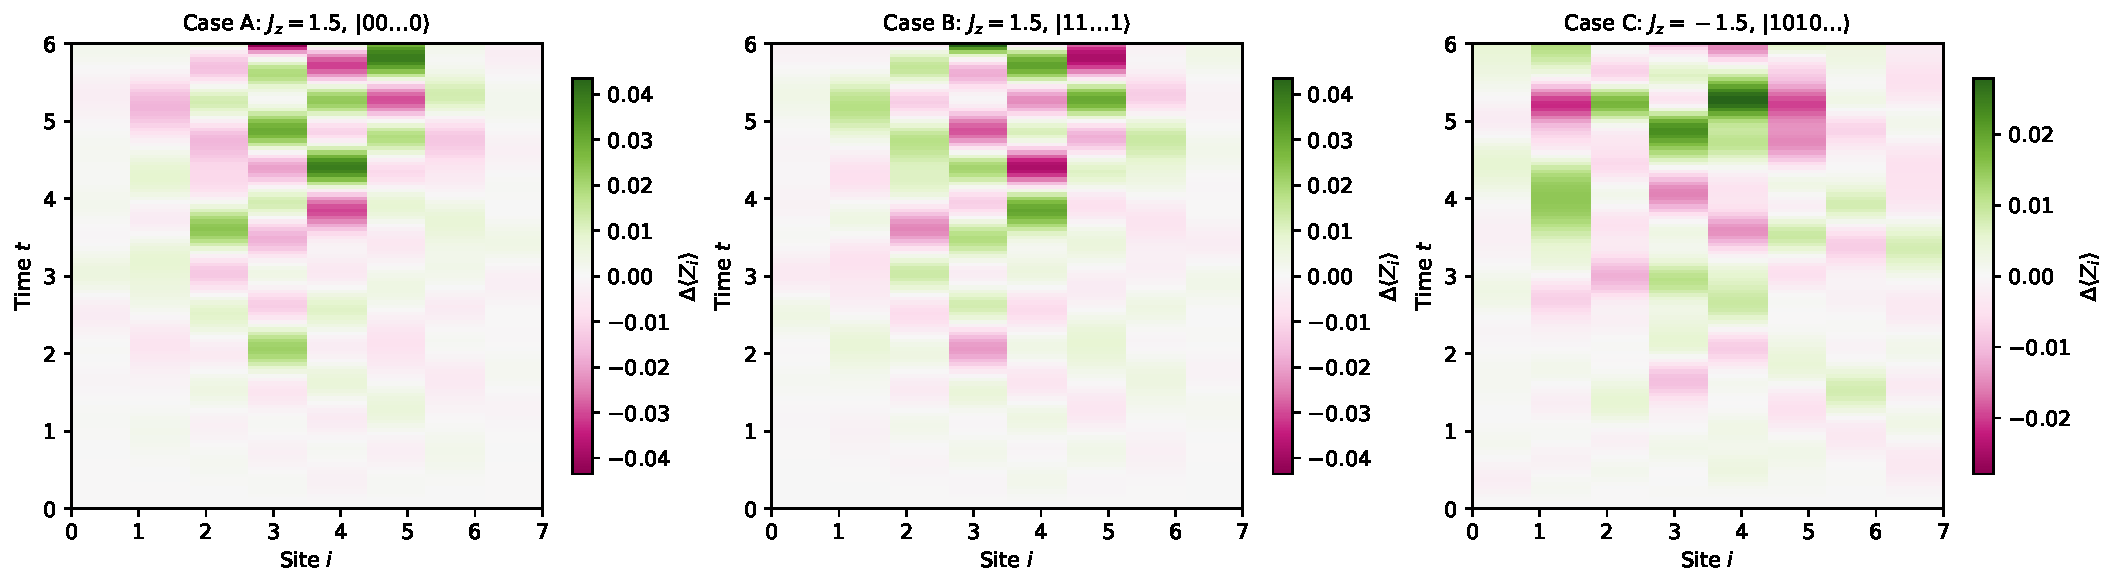
\includegraphics[width=0.9\textwidth]{figures/trotter_error.pdf}
    \caption{\textbf{Residual error of the ideal Qiskit second-order Trotter simulation.} The heatmaps display $\Delta\langle Z_i(t) \rangle = \langle Z_i(t)\rangle_{\text{Qiskit}} - \langle Z_i(t)\rangle_{\text{Exact}}$. Maximum deviations occur at the boundaries of the light cone at late times, characteristic of the compounding nature of product-formula truncation errors.}
    \label{fig:trotter_error}
\end{figure}

\subsection{Error Scaling Analysis}
A fundamental validation of the algorithmic implementation is the convergence of the Trotter approximation with decreasing $\Delta t$. Figure \ref{fig:error_scaling} illustrates the state infidelity and observable root-mean-square error (RMSE) as a function of the number of Trotter steps. 

\textit{Due to the global spin-flip symmetry of the XXZ Hamiltonian, the dynamics and resulting Trotter errors for Case A (all-down) and Case B (all-up) are numerically identical. To avoid redundant overlap, the data for Case B has been omitted from the plot.}

% Placeholder for Error Scaling Figure
\begin{figure}[h]
    \centering
    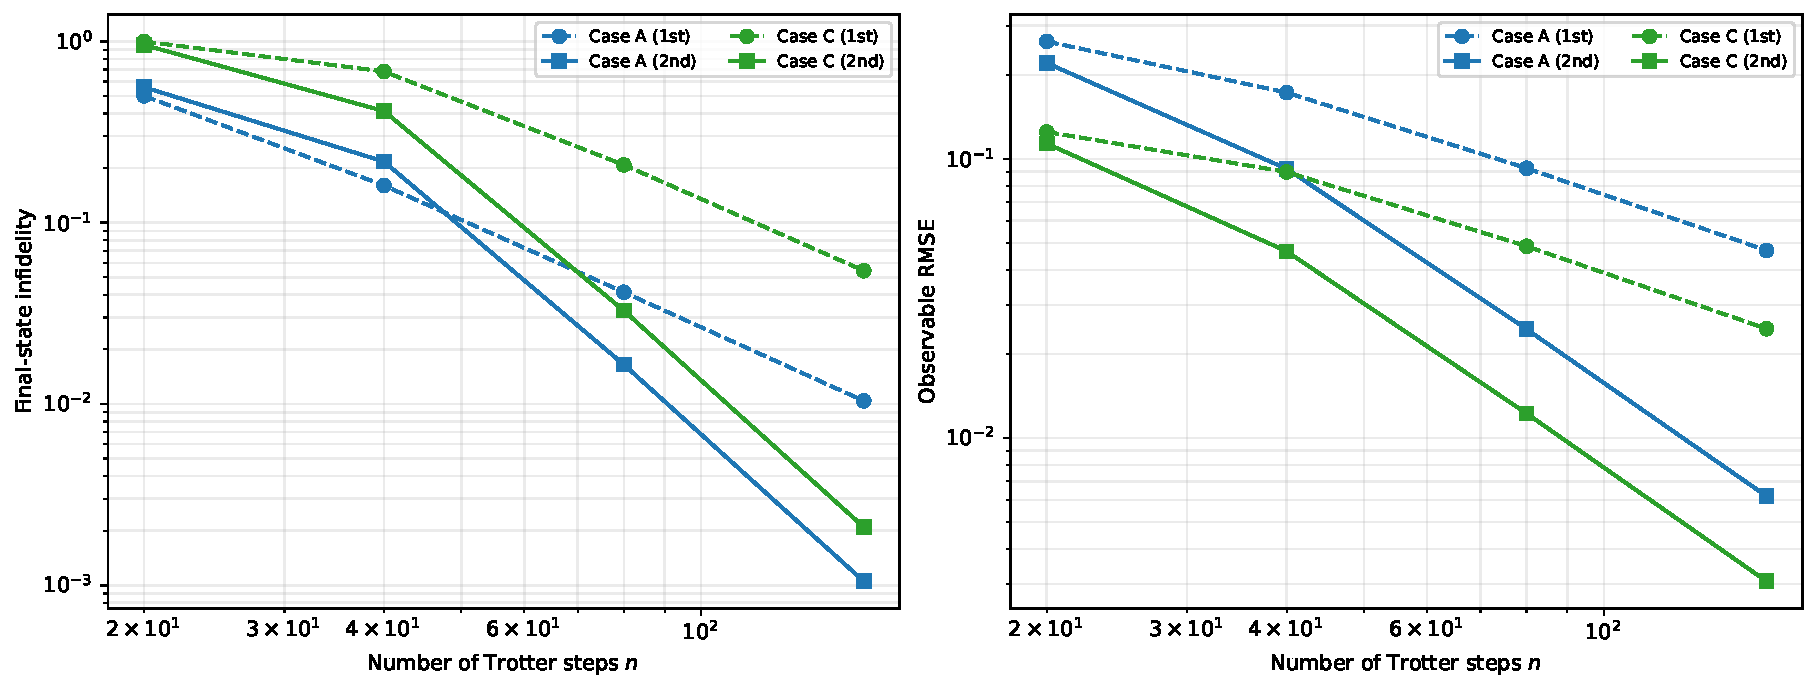
\includegraphics[width=0.8\textwidth]{figures/error_scaling.pdf}
    \caption{\textbf{Trotter error convergence (1st vs. 2nd order).} Both final-state infidelity and observable RMSE decrease monotonically as the number of Trotter steps increases. The steeper slope of the solid lines verifies the superior $\mathcal{O}(\Delta t^3)$ local scaling of the symmetric second-order decomposition compared to the first-order approach.}
    \label{fig:error_scaling}
\end{figure}

\subsection{Noisy Simulation Results}
Figure \ref{fig:noisy_dynamics} contrasts the ideal exact dynamics with the \texttt{AerSimulator} density-matrix results subject to gate noise. While the short-time ballistic propagation is preserved, late-time ($t \gtrsim 4$) interference patterns are significantly blurred, representing a loss of quantum coherence. The RMSE increases by over an order of magnitude (from $\sim 10^{-2}$ in the ideal case to $\sim 10^{-1}$ in the noisy regime).

% Placeholder for Noisy Dynamics Figure
\begin{figure}[h]
    \centering
    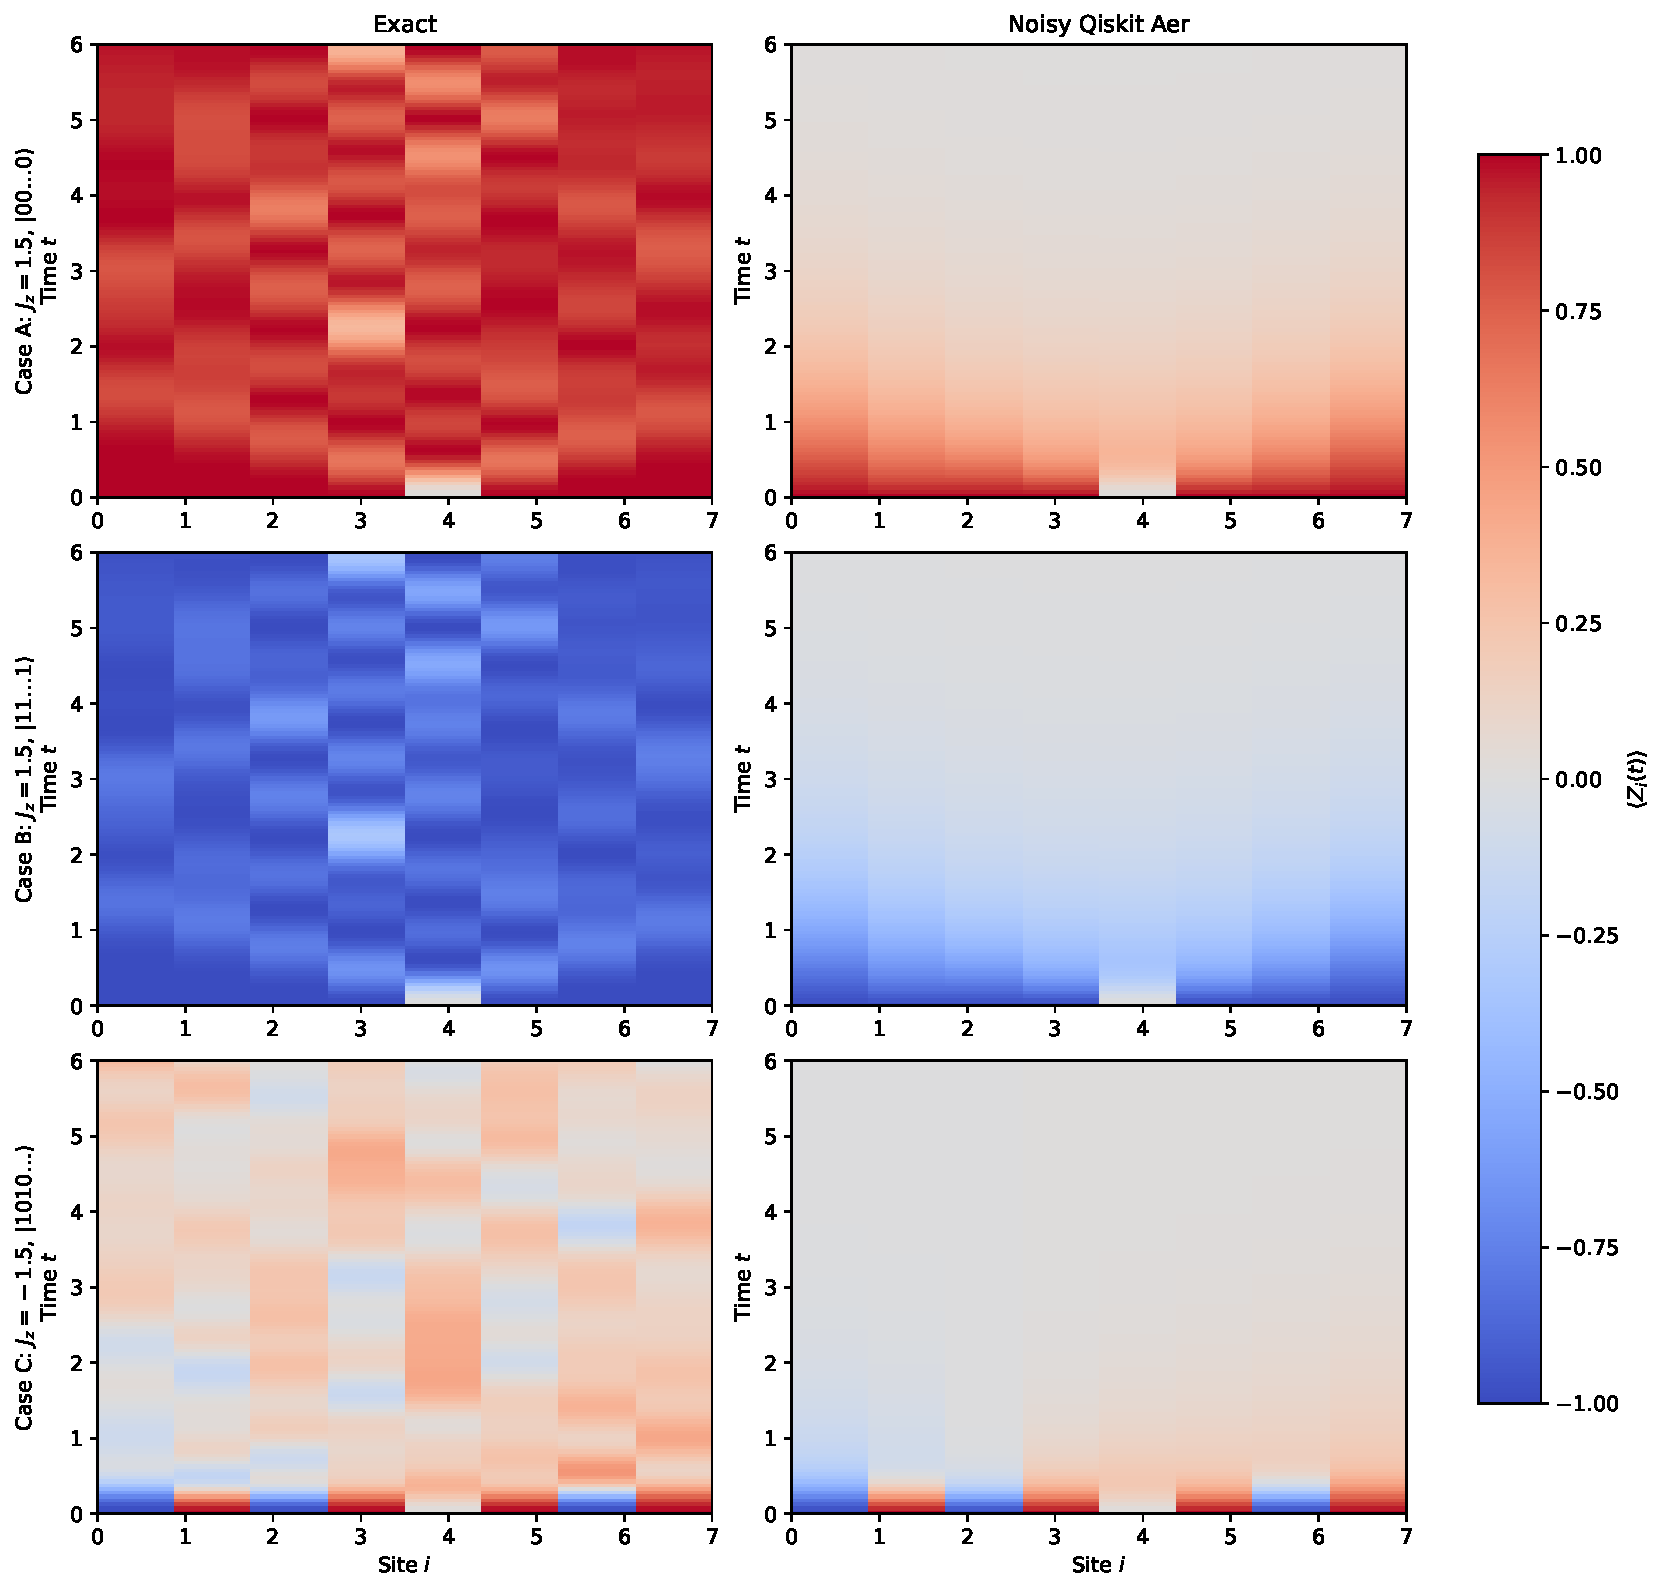
\includegraphics[width=0.8\textwidth]{figures/noisy_dynamics.pdf}
    \caption{\textbf{Impact of gate noise on $\langle Z_i(t) \rangle$ dynamics.} Exact dynamics (left) are compared with noisy Qiskit Aer simulations (right) ($p_X = 0.002, p_Z = 0.006$). Noise acts as a highly effective decoherence mechanism, damping the oscillatory spin-wave signals and driving the local magnetisation towards a uniform mixed state.}
    \label{fig:noisy_dynamics}
\end{figure}

\subsection{Spectral Analysis}
To interpret the collective excitations (magnons), we perform a 2D discrete Fourier transform on the mean-subtracted magnetisation field, $|\mathcal{F}_{2D}[\langle Z_i(t)\rangle - \overline{\langle Z\rangle}]|$, projecting the data into the momentum-frequency $(k, \omega)$ domain (Figure \ref{fig:spectra}). 
\textit{Note that the momentum resolution is fundamentally limited by the finite system size ($L=8$), yielding exactly 8 discrete $k$-modes.}

% Placeholder for Spectral Analysis Figure
\begin{figure}[h]
    \centering
    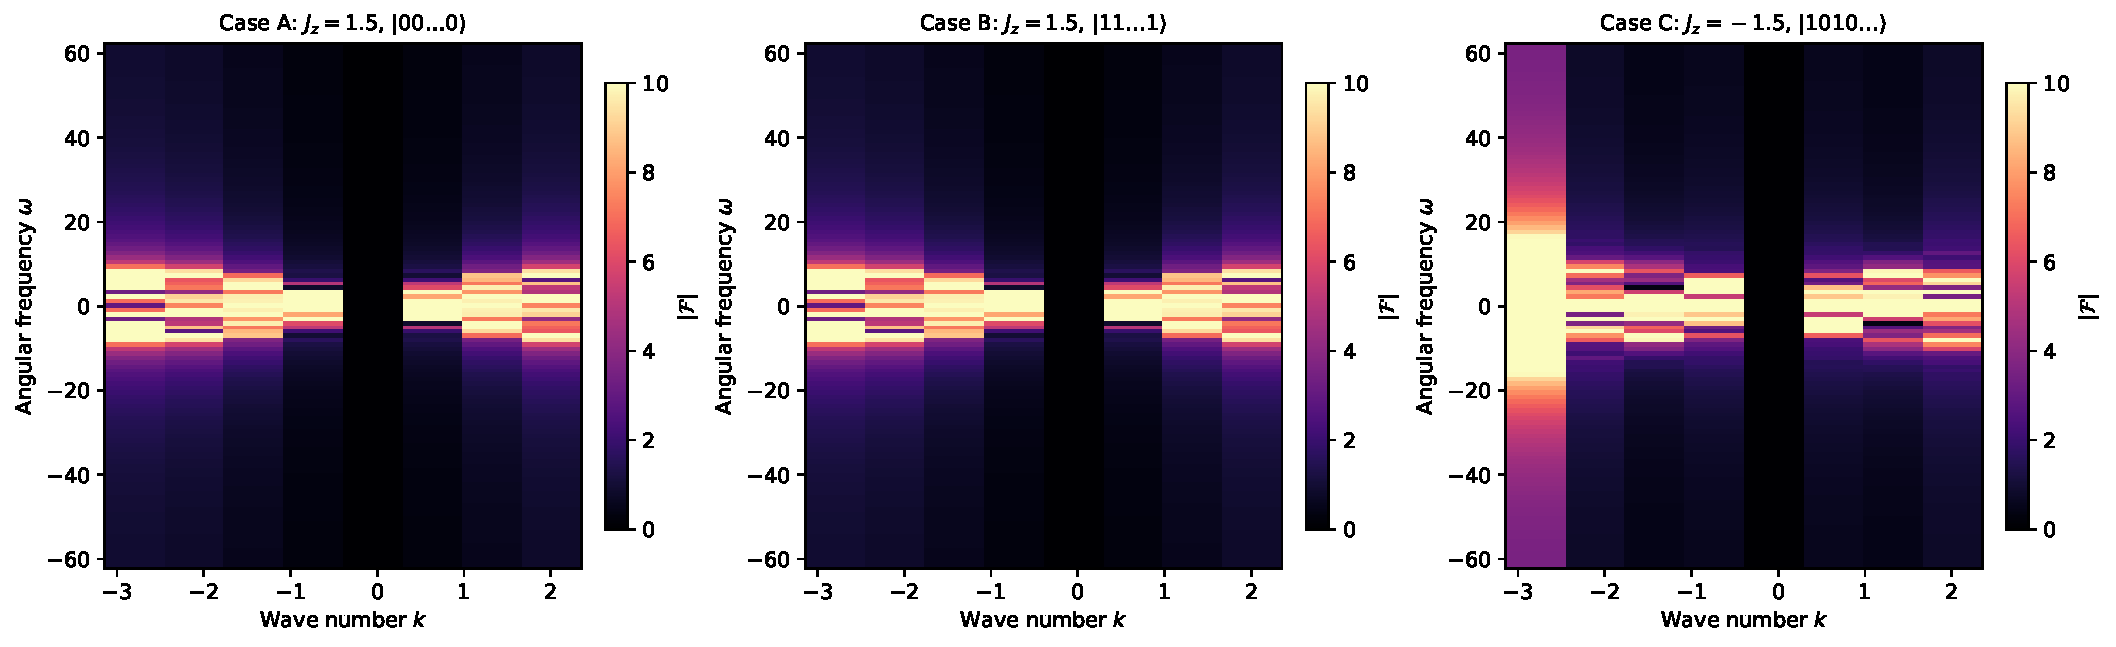
\includegraphics[width=0.9\textwidth]{figures/spectra.pdf}
    \caption{\textbf{Momentum-frequency spectra of $\langle Z_i(t)\rangle$.} The dispersive features represent the magnon branches of the system. Cases A and B exhibit spectral weight near $k=0$, typical of long-wavelength ferromagnetic excitations. Case C displays concentrated intensity near the Brillouin zone boundary ($|k| \sim \pi$), consistent with the underlying N\'eel order.}
    \label{fig:spectra}
\end{figure}

% ====== 6. Discussion ======
\section{Discussion} \label{sec:discussion}

\subsection{Methodological Trade-offs and Noise Limitations}
Our investigation delineates three distinct tiers of simulation fidelity. Exact sparse evolution serves as an immaculate ground-truth but is fundamentally unscalable. Ideal Qiskit Trotterisation accurately reproduces the many-body dynamics, confirming that circuit-level approximations are theoretically robust provided the order of the product formula is appropriately matched to the time step. 

However, the introduction of realistic gate noise rapidly overtakes the theoretical Trotter error. The noisy density-matrix simulations clearly demonstrate that for near-term superconducting or ion-trap architectures, suppressing physical decoherence is a far more pressing bottleneck than selecting higher-order algorithmic decompositions. The exponential decay of late-time signal fidelity highlights the necessity for advanced error mitigation strategies (e.g., zero-noise extrapolation, randomized compiling \cite{Campbell2019}) or full quantum error correction before deep Hamiltonian simulations can achieve practical utility.

\subsection{Physical Interpretation}
The quantum simulations consistently confirm the predicted ballistic propagation of local perturbations governed by the Lieb-Robinson bounds of the XXZ Hamiltonian. The distinct signatures in the momentum-frequency spectra validate that our initial local $R_z$ rotation successfully excites the characteristic magnon modes. The symmetry between the ferromagnetic all-up and all-down states acts as a powerful sanity check on the parity conservation within the Qiskit Trotter operators, while the antiferromagnetic N\'eel case correctly highlights high-frequency, short-wavelength interactions.

\subsection{Scaling Outlook}
While classical exact diagonalisation handles $L=8$ with trivial ease, ensuring zero "quantum advantage" in this specific domain, this scale is optimal for rigorous pedagogical benchmarking. The true strength of the Trotter circuit formalism lies in its linear scaling in spatial and temporal resources. As experimental coherence times improve, extending this circuit architecture to $L \gtrsim 50$ spins will rapidly transition the problem out of the classical simulation regime, representing a critical frontier for near-term quantum utility \cite{Kim2023}.

% ====== 7. Group Organisation ======
\section{Group Organisation} \label{sec:group}
% TODO: Add group organisation, task allocation, and collaboration strategies here.

% ====== 8. Applications ======
\section{Applications} \label{sec:applications}

The framework implemented in this study extends significantly beyond the pedagogical exercise of simulating spin chains. The ability to map fermionic or bosonic operators onto Pauli matrices (e.g., via Jordan-Wigner transformations) implies that these precise Hamiltonian simulation techniques are directly applicable to modeling strongly correlated electron systems, such as high-$T_c$ superconductors described by the Hubbard model.

Furthermore, the simulation of real-time dynamics holds immense potential for non-equilibrium physics and Lattice Field Theories (LFTs). While classical Markov Chain Monte Carlo (MCMC) methods struggle with the infamous "sign problem" when simulating real-time evolution or systems at finite chemical potential, quantum circuits naturally handle complex amplitudes. As such, expanding the Trotterized circuits developed here serves as a stepping stone toward calculating dynamic scattering cross-sections and real-time evolution in quantum chromodynamics (QCD).

% ====== 9. Conclusion ======
\section{Conclusion} \label{sec:conclusion}

This project successfully modelled the real-time dynamics of the XXZ Heisenberg spin chain using classical exact diagonalisation and quantum circuit simulations. We demonstrated that a second-order Trotter-Suzuki decomposition implemented via Qiskit faithfully captures the complex spin-wave propagation and spectral features of the system with $\mathcal{O}(\Delta t^3)$ precision. 

Crucially, by incorporating a density-matrix noise model, we quantitatively showed that modern gate-level imperfections rapidly dominate algorithmic errors, heavily damping quantum coherence at late times. This dual perspective—confirming the theoretical viability of the quantum algorithm while exposing its current hardware vulnerability—provides a robust, academically rigorous evaluation of Hamiltonian simulation in the NISQ era. Future work must integrate these simulation frameworks with error mitigation protocols to bridge the gap between theoretical algorithms and scalable physical deployment.

% ====== References ======
\begin{thebibliography}{9}

\bibitem{Georgescu2014}
I. M. Georgescu, S. Ashhab, and F. Nori, ``Quantum simulation,'' \textit{Rev. Mod. Phys.} \textbf{86}, 153 (2014).

\bibitem{Daley2022}
A. J. Daley \textit{et al.}, ``Practical quantum advantage in quantum simulation,'' \textit{Nature} \textbf{607}, 667 (2022).

\bibitem{Feynman1982}
R. P. Feynman, ``Simulating physics with computers,'' \textit{Int. J. Theor. Phys.} \textbf{21}, 467 (1982).

\bibitem{Lloyd1996}
S. Lloyd, ``Universal quantum simulators,'' \textit{Science} \textbf{273}, 1073 (1996).

\bibitem{AlMohy2011}
A. H. Al-Mohy and N. J. Higham, ``Computing the action of the matrix exponential, with an application to exponential integrators,'' \textit{SIAM J. Sci. Comput.} \textbf{33}, 488 (2011).

\bibitem{Krantz2019}
P. Krantz \textit{et al.}, ``A quantum engineer's guide to superconducting qubits,'' \textit{Appl. Phys. Rev.} \textbf{6}, 021318 (2019).

\bibitem{Campbell2019}
E. Campbell, ``Random compiler for fast Hamiltonian simulation,'' \textit{Phys. Rev. Lett.} \textbf{123}, 070503 (2019).

\bibitem{Kim2023}
Y. Kim \textit{et al.}, ``Evidence for the utility of quantum computing before fault tolerance,'' \textit{Nature} \textbf{618}, 500 (2023).

\end{thebibliography}

\end{document}